\documentclass{inets-thesis}

% For editing the LaTeX environment, refer to owndefs.tex. Don't edit the inets-thesis.cls file!

% Title of the thesis
\ThesisTitle{Visualization of Radio Networks in a Three Dimensional Environment}

% Thesis type ("M" = master thesis, "B" = bachelor thesis)
\ThesisType{B}

% Author's name (firstname(s) lastname)
\ThesisAuthor{Markus Stroot}

% Date (year month day)
\ThesisDate{2016}{11}{23}

% Examiners: Check who is your first examiner from our professors.
% There is always one first examiner (listed in your registration sheet), and one more examiner
% who in our case is usually the respective other professor, supervisors are non-faculty members
% who supported you in addition to the first examiner in the development of the thesis
% Advisers: Reference with name and title, note that old German titles (Dipl.-Ing.) and doctor titles (Dr. or % Dr.-Ing.) are prefix while ``M.Sc.'' is a postfix to the name of the person

\FirstExaminerName{Prof.~Dr.-Ing.~Marina Petrova}
\SecondExaminerName{Prof.~Dr.~Petri M\"ah\"onen}
\SupervisorNames{Dr.~Ljiljana Simi\'{c}\\Dr.-Ing.~Janne Riijij\"arvi}

\begin{document}

\chapter{Introduction}
In today's world, mobile communication has become extremely popular and highly essential to the social and economical part of our society. Nearly every person living in the industrial countries possesses at least one device capable of wireless communication of some sort. The high density of mobile devices in urban areas has lead to some interesting challenges in the planning and implementation of wireless network infrastructure. On the one hand, the network needs to be able to manage the high data throughput that is created by hundreds or thousands of devices. On the other hand, the network quality needs to be acceptable at any point in the area, because a high throughput is useless if the devices cannot access the network efficiently.

The network coverage problem is especially interesting in urban areas, because of the unique topology. Devices may be mounted atop a very tall skyscraper or far down in the streets, surrounded by buildings. Most of the commonly used wireless communication systems use electromagnetic waves to deliver information, which is no problem on a plane field. Within the rising and falling topology of an urban area however, the propagation of the network gets more difficult to predict. Just like it is with light, obstacles made of different material can absorb, reflect, alter or do nothing to any passing electromagnetic wave. This causes areas of high signal strength, where the antenna has a direct line of sight or a good reflecting path. However, it also crates areas of poor signal strength, for example behind a building (shadow) or in places, where reflections cause too much interference. Over time research institutions have addressed the problem and developed models to predict how network propagation behaves in obscured or confined areas. Many methods however are far to complex to be evaluated by hand for any realistic scenario. Hence, computer supported network simulation emerged. With the help of the computing power of modern computer programs like the WinProp Software Suite~\cite{WinProp} are able to forecast the behavior of wireless networks in different environments. Modern simulation applications can predict network propagation for large areas and many different antennas at the same time with decent accuracy. These tools provide a helpful overview over the network coverage, which is especially important for the current trend of infrastructure development.

Currently, the focus is shifting, when it comes to the design of wireless or radio networks in particular. Big macro cells, which provide efficient coverage in rural areas, often struggle in more urban areas, because of the way the buildings interact with the electromagnetic waves. Therefore big cell are being split up, to enhance throughput and directional preferences. Furthermore, newly installed cells are often micro cells, tailored to a specific location in performance and directional properties. This trend however makes it harder to plan where and how to install new infrastructure nodes, in order to satisfy demands. It takes careful analysis of wide range simulations and real life measurements to identify weak points in the coverage and patch them up or to increase signal quality in very demanding areas.

This is where good visualization applications come into play. There are already some tools (e.g. as part of WinProp~\cite{WinProp}) that try to help developers by visualizing the signal strength of simulated network scenarios. However, those mainly work in two dimensional space. From a top down perspective the network propagation is shown for a fixed height parameter. This can be helpful for engineers and developers. However, a realistic three dimensional representation of the environment with buildings, maps and the network propagation in between would be even more convenient. Any spacial arrangements and their problems would be easily viewable. For that reason, this thesis tries to first point out the challenges and prerequisites in creating a useful and user-friendly network visualization tool. Thereafter a possible implementation is presented. Finally, the application is analyzed, evaluated and expanded upon.
\chapter{Three Dimensional Visualization and Web Development}

As any software project, this visualization tool also relies on many different algorithms and technical standards or conventions. This chapter aims to give an overview of the major external components and ideas, that contribute to the project and the way it works.
\section{Algorithms}
\subsection{Marching Cubes Algorithm} \label{chp2:Cubes}
The marching cubes algorithm was designed in 1987 and published in \cite{MarchCubes}. The original idea was to create high resolution triangle models of constant density surfaces for medical purposes. However, the algorithm can be applied to any three dimensional scalar data set, not only tissue density. The aim of the algorithm is to find an isosurface within a data set. An isosurface is a two dimensional surface within a three dimensional context, that connects the points in space in which the data set has the same value.\footnote{Compare contour lines on a two dimensional map.}

The algorithm uses the ``divide and conquer'' approach. It divides the whole set into small cubes, which it then iterates or `marches' through. The cubes are evaluated at the corners and each one gets marked, if it exceeds the isosurface value $val_{iso}$. That leads to $2^8=256$ different ways for a cube to be marked. Based on the marked corners, triangles are inserted within the cube, so they separate the marked corners from the unmarked ones. This is a clever way, because if a corner with a higher value is adjacent to one with a lower value, the isosurface has to intersect the edge somewhere in between. In order to further enhance the accuracy of the surface, a linear interpolation is used, to decide where on each edge of the cube the corners of the triangle(s) should be placed. Using two different symmetries the actual number of triangle arrangements can be reduced to 14. In each of those there is up to four triangles, as can be seen in figure \ref{fig:cubes-arr}.
\begin{figure}\begin{center}
  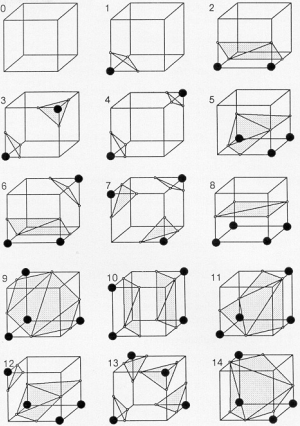
\includegraphics[width=0.45\textwidth]{pictures/cubes_arrangements}
  \caption[Tringles arrangements]{Tringles arrangements. as seen in \cite{MarchCubes}}\label{fig:cubes-arr}
\end{center}\end{figure}

Most implementations of the Marching Cubes Algorithm use lookup tables to store which edges get intersected, based on the marked corners. This makes sense, since an array lookup is a very cheap instruction, when it comes to processing time and an array with 256 entries usually is not too big. Especially in comparison to the number of triangles that is needed for a satisfying reconstruction of any realistic 3D-surface.

\section{File Types}
\subsection{Shapefile}
A shapefile stores attribute and geometry information. Geometries are represented by shapes consisting of a set of vector coordinates. As it can be seen in its technical description~\cite{ersi:shp} a shapefile actually consists of more than one file. There are at least three parts to every shapefile. A main file, an index file and a dBASE table. The files are all named by the same valid filename. The suffix however distinguishes between the main (.shp), the index (.shx) and the dBase (.dbf) files.

The main file grants direct access to the geometrical information. It consists of a \unit[100]{byte} header followed by variable-length records. The header contains file management information, like the file code, file length, etc. It also gives information on the data set, like bounding box coordinates and shape type. The records represent the actual shapes. Each record consists of an \unit[8]{byte} record header and a variable sized list of vertices. The record header simply contains the record number and its length. The length depends on what shape is represented and how many vertices it is made up of. The organization of the main file can be seen in figure~\ref{fig:main-orga}.
\begin{figure}\begin{center}
  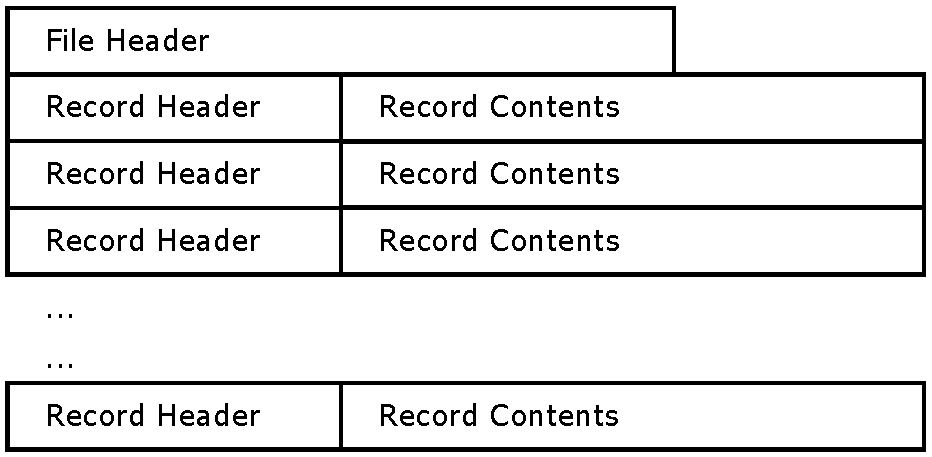
\includegraphics[width=0.8\textwidth]{pictures/Shapefile}
  \caption[Organization of the Main File]{Organization of the Main File. as seen in \cite{ersi:shp}}\label{fig:main-orga}
\end{center}\end{figure}

The index file also starts with a \unit[100]{byte} header, which is identical to the main file header. After that, there is a record entry for each of the records in the main file. The $i^{th}$ record entry contains the length of the $i^{th}$ record in the main file and its offset relatively to the beginning of the file.

The dBASE file contains additional attributes concerning the shapes. The format is a standard DBF file, that is used by many applications with only a few extra requirements. The record order for example has to be the same as the order of the shapes in the main file.

\subsection{ODA files}
The ODA file format is a simple way to to store geometrical information about urban outdoor environments. This format is especially interesting, because it is used by the WallMan~\cite{WallMan} application in the WinProp wireless network planning software package~\cite{WinProp}. It is a simple ASCII format.

The file starts with a header of six lines, consisting of five lines of comment and one line of general database settings. The body of the file consists of two blocks. The first block contains some material information, which is  referred to in the second block. That block holds the actual outdoor building data. All buildings are represented by an arbitrary number of 2D-coordinates, outlining the base shape, and one height parameter.

\subsection{APA file}
The APA file format is an ASCII based format used by the AMan~\cite{AMan} application, which is also part of the WinProp wireless network planing software package~\cite{WinProp}. It stores three dimensional antenna gain patterns. APA files mostly consist of data triples. There can only be one triple per line and it must be made up of two angular values (horizontal and vertical) and one gain value (in \unit{dB}).

\subsection{CSV file}
The CSV~\cite{CSV} file format is a widely used, ASCII based, format. It is able to represent any kind of tabular data. Different characters can be used to separate the data values. The line break character usually signifies the end of a data record. Within each record there can be multiple data fields, separated by a special character\footnote{The comma is usually used for that, but semicolon, colon, tab or space are alternatives.}.

\section{Rendering and Output}
\subsection{Rendering Basics}
\subsection{Three.js WebGL Framework}
Three.js is a JavaScript based API\@. It uses WebGL~\cite{WebGL}. Therefore it provides the opportunity to use hardware accelerated 3D-graphics inside of HTML5 browsers, making it platform independent.

The framework was first published in 2010 by Ricardo Cabello, also called {``mrdoob''} online.~\cite{ThreeWhite} He started with 3D modeling and editing together with other programmers. When he felt, that the tools he used to create his animation scenes were not satisfying his needs, he started do develop his own framework. When finally JavaScript and WebGL support started to get better, he ported this project from ActionScript to JavaScript an published it on GitHub\footnote{available on: https://www.github.com/mrdoob/three.js}. Since then many contributors are still taking part in the development of that project.

The aim of the framework is to abstract the work and theoretical calculations, that come up when a three dimensional scene is rendered to a two dimensional screen. It provides developers with classes and methods that are convenient for the fast and easy creation of three dimensional scenes. Implemented are many usefull features~\cite{ThreeFeatures} like:
\begin{description}
\item[Different Renderes] are available, including WebGl, Canvas and SVG renderer
\item[Scenes] can be edited at run-time
\item[Cameras and Controllers] in many different varieties.
\item[Lighting] can be added to a scene like any object; Shadows are calculated internally
\item[Materials] with different shadow and texture options are provided.
\item[Geometries] both custom made and predefined (cube, sphere, torus, \ldots)
\item[Loaders] for images, JSON objects and more
\item[Examples] are provided on nearly every functionality the framework provides
\end{description}
All this lets the developers working with three.js focus more on designing an creating the scene, rather than on the difficulties of displaying it on the computer screen. However, should a special case arise and the developer needs to work on a more basic level, that is no problem. Three.js can incorporate any self-written shaders and posses a variety of utility math functions, like matrix and vector calculation and projection.

Listing~\ref{list:example} shows an easy example on how to use three.js in a JavaScript document. The code creates a Scene, a PerspectiveCamera, and a WebGLRenderer object. The renderer is then added to the body of the HTML page. Afterwards the predefined BoxGeometry and MeshBasicMaterial classes are used to create the mesh of a simple 1x1x1 cube. Finally, it is added to the scene and the camera is moved. Now the rendering loop is started, which slowly rotates the cube around the x and y axis. This example shows how a relatively complex animation can easily be implemented with just a few lines of code.
\lstset{
caption=Three.js Example,
label=list:example,
language=JavaScript}
\begin{lstlisting}
var scene = new THREE.Scene();
var camera = new THREE.PerspectiveCamera( 75, window.innerWidth / window.innerHeight, 0.1, 1000 );

var renderer = new THREE.WebGLRenderer();
renderer.setSize( window.innerWidth, window.innerHeight );
document.body.appendChild( renderer.domElement );

var geometry = new THREE.BoxGeometry( 1, 1, 1 );
var material = new THREE.MeshBasicMaterial({
	color: 0x00ff00
	});
var cube = new THREE.Mesh( geometry, material );
scene.add( cube );
camera.position.z = 5;

function render() {
	requestAnimationFrame( render );
	
	cube.rotation.x += 0.1;
	cube.rotation.y += 0.1;

	renderer.render( scene, camera );
}
render();
\end{lstlisting}

\subsection{Possible Renderman Pipline (?)}
\chapter{System Architecture}
\section{System Requirements}
\subsection{Hardware Requirements}
One of the most important hardware elements for the three dimensional visualization is the graphics~card\footnote{In some cases the hardware acceleration is disabled. See Section \ref{SoftReq} for further information.}. Depending on the size and level of detail of the scene there are a lot of computations that need to be done. Furthermore, the scene is supposed to be movable, so it cannot be a prerendered image. That makes some dedicated graphics hardware nearly indispensable. However, since the application renders simple polygon meshes and point clouds the graphics hardware does not have to be a high end device. It merely needs to relieve the CPU of some work. And with its processing unit made especially for matrix and vector calculation, any modern day graphics card that supports WebGL will meet the expectations.

CPU-only rendering is of course possible, too. The large amount of of points and surfaces in a complex scene however seriously slows down the rendering on an all purpose CPU. This also slows down the whole system, because of all the graphics calculations that are blocking the CPU. For a more detailed analysis see Section \ref{test}.

Another important hardware requirement is the RAM. Visualization data sets, especially from simulation applications, can get large very fast. City wide simulations with multiple antennas and a resolution of a few meters can easily have a few million data points. While the data that is being visualized might not take up much space as a file on the hard drive, within the application that might change. After being loaded and parsed, the data is stored within convenient data structures like arrays or objects. This leads to a less efficient compression of the data and also the addressing schemes and object methods add additional overhead. All that together results in an application that needs to load big chunks of data into the RAM. Therefor it is important that the system has enough memory at its disposal.
\subsection{Software Requirements} \label{SoftReq}
Since the main routine of the application, the rendering loop, runs in a web browser as JavaScript code, it is important to have a browser, that supports all the used functionality. Firstly, and most importantly, the renderer used here is a so called ''webGL-renderer´´, so it is important that the browser even supports WebGL. All current versions of the commonly used ones (e.g. Chrome, Firefox, Safari, \ldots) are able to support HTML5, CSS3 and WebGL. It is advisable to use the most recent update of the browser, because the developers always improve the performance or fix bugs. Also the support of WebGL grew over time, so very old versions may not support all the features used in this application. For lesser known browsers the functionality has to be determined individually. Important criteria are the former mentioned HTML5, CSS3 and WebGL support. It is also worth mentioning that the browser needs to allow WebGL to use hardware accelerated rendering, in other word access the graphics card. Microsoft's Internet Explorer for example does not do that. This leads to the problem, that it uses CPU-only rendering even if a graphics card is installed, which in turn, slows down the whole system.
\section{Architectural Design}
\subsection{Initial JavaScript code}
\subsection{Frontend -- Backend}
\chapter{Implementation}
\section{Datastructures}
Within the implementation the data needs to be represented in a way, that is convenient for the algorithms to work on. In this section I will present some of the special datastructures.
\subsection{Four Dimensional Arrays}
The four dimensional array in itself is not an exceptional datastructure, but it has a special meaning in this application. The data delivered by simulation application usually comes as values that can be indexed by the three spacial definitions that define its location.Furthermore, in many simulation circumstances there is more than one antenna, so you get multiple power values for each point in space. Hence, the four dimensional array is a good was to represent this data. In this application, the first index represents the number of the antenna or base station, while the other three indices represent the three spacial directions. Of course, this only works for evenly spaced  positions, but since the marching cubes algorithm works best on evenly spaced data points, this restriction is sensible either way.
\subsection{Data Point Object}
The other way to represent data is used for real life measurement data. Here you cannot expect the points to be evenly spaced. They mostly follow streets, or other easily accessible places. Therefore we need exact information on the location of each point. This is realized by a very simple point-object in JavaScript. It has only three members, the x coordinate or ?? and the y coordinate or ??. This is useful for the inverse distance interpolation used for the real data, because you can easily calculate the distance to any point in space.

A very similar object is used to represent the antenna patterns. Those patterns consist of a horizontal angle, a vertical angle and a amplification for the corresponding direction. Hence, in this case, two of the members represent a direction rather than a point and the value equals the amplification.
\section{Important algorithms and routines}
This section describes some classes or functions in either backend or frontend code that implement the core functionality of the application.
\subsection{The Ajax Loader}
The Loader-class is a JavaScript object. It encapsulates four methods, that provide requests for the four different types of data, that are needed in this application. Namely those are building data, measurement data, simulation data and antenna patterns.

\lstset{
caption=Building Loader,
label=list:Loader,
language=JavaScript}
\begin{lstlisting}[float=bph]
GuiInterface.prototype.loadBuildings = function (path) {
    var uri = 'api/Building/Get/' + path.replace(".", ";");
    $.ajax({
        url: uri,
        type: "GET",
        datatype: "json"
    })
    .done(function (data) {
        var Build = new BuildingLoader();
        Build.addBuild(data);
    })
    .fail(function (a, b, c) {
        alert("Error")
    });
};
\end{lstlisting}

Listing \ref{list:Loader} shows the exemplary implementation of the building loader method. Forming a request is very straight forward. The \$-identifier grants access to the methods provided by the JQuery library. There the `ajax' method abstracts a generic server request. In the curly braces afterwards, one simply has to specify the options. The `url' option sets the request url. This is important because it determines which controller the request is mapped to. The  `type' option tells the server what kind of request is send. Requests to retrieve data usually use the `GET' method. Finally, the `datatype' option tells the server, what kind of response is expected. Since this application mostly requests objects, it expects a response that contains a JSON object. The next methods define callback-functions that get executed on specific events. The `done' method gets executed when the request returns successful, while the `fail' method executes on any error that gets returned.

Each of the loader methods has an individual `done' method. Depending on the type of data that is loaded, those methods creates a specific class instance, which is able to create a three dimensional representation of the data and puts it into the scene. In the case of Listing \ref{list:Loader} the BuildingLoader class uses the method `addBuild' and passes the newly retrieved building data.


\subsection{Filling Simulation data}
Data that gets provided by some Simulation tool, like WinProp~\cite{WinProp}, usually has an overall uniform structure. This means that it consist of points in three dimensional space and one or more power values for each point. Furthermore, those points have a uniform spacing per dimension. However, the three dimensional scalar field can have holes, when buildings or other obstacles are in the way or the antenna is really far away. In that case these holes need to be filled, so the Marching Cubes Algorithm will work properly. This operation is not depending on any graphical calculations, so it is done by the backend directly after reading the data. Listing shows the C\# method, that does this. 
\lstset{
caption=Building Loader,
label=list:Fill}
\begin{lstlisting}[language=C, float=bph]
public void fill()
        {
            double xdiff = 0, ydiff = 0, zdiff = 0;
            double lastx = x[0];
            double lasty = y[0];
            double lastz = z[0];
            bool boolx = true, booly = true, boolz = true;

            for (int l = 0, m = 0; l < x.Count; l++) {
                if (lastx != x[l] && boolx) {
                    xrang = m++;
                    xdiff = Math.Abs(lastx - x[l]);
                    boolx = false;
                }
                if (lasty != y[l] && booly) {
                    yrang = m++;
                    ydiff = Math.Abs(lasty - y[l]);
                    booly = false;
                }
                if (lastz != z[l] && boolz) {
                    zrang = m++;
                    zdiff = Math.Abs(lastz - z[l]);
                    boolz = false;
                }
                if (!boolx && !booly && !boolz)
                    break;
                if (l == x.Count - 1) {
                    if (m < 2)
                        throw new System.Exception("no valid values");
                    if (boolx)
                        xrang = 2;
                    if (booly)
                        yrang = 2;
                    if (boolz)
                        zrang = 2;
                }
            }
            for (int l = 0; l < x.Count; l++) {
                if (Math.Abs(lastx - x[l]) > xdiff && l % (xlookup[xrang, yrang] * dim[0]) != 0)  {
                    introduce(l, lastx, xdiff, 'x');
                    l--;
                }
                if (Math.Abs(lasty - y[l]) > ydiff && l % (ylookup[yrang, zrang] * dim[1]) != 0) {
                    introduce(l, lasty, ydiff, 'y');
                    l--;
                }
                if (Math.Abs(lastz - z[l]) > zdiff && l % (zlookup[zrang, xrang] * dim[2]) != 0) {
                    introduce(l, lastz, zdiff, 'z');
                    l--;
                }
                lastx = x[l];
                lasty = y[l];
                lastz = z[l];
            }
        }
\end{lstlisting}

After reading the data from a file, all data points are in one big array with coordinates and values. Therefore we can just go through the array and fill in the missing values. The first for loop determines how much the spacing is and which order the coordinates have within the global order. It checks in every run, if the x, y or z coordinates have changed. If one changes, it gets the next higher rank (from 0 -- 2) with the help of the global rank counter `m'. This ensures, that the order in which the dimensions are iterated through by the simulation can be arbitrary. Further, the difference between the changing coordinates gets saved as the corresponding step width. The boolean variables simply interrupt the routine, if all three ranks have been determined. If the loop runs through on the last element of the array, that means there has to be at least one dimension, which has just a single value for coordinates, making the data at least two dimensional. In that case variable m gets evaluated. A value of 1 means that only one dimension has changing coordinates, therefore the system would be one dimensional. That does not make any sense for a visualization, so an error gets thrown. In the case of $m=2$ the data is two dimensional, which is not ideal, but may be visualized as a plane. The remaining variable gets a rank of 2.

The complicated part follows in the next for loop. Here the function again runs through the array, but now it actually fills up the holes. There are two conditions that have to be met, in order to detect a hole. Condition number 1 states that a possibles hole occurs, where the difference of the last value for that coordinate and the current value is greater than the previously determined step width. The second condition is necessary, because the values will also jump at the end of the data set in that direction. In other words, the distance between  three dimensional indices within the global array cannot be a divisor of the current index. The distance of the indices is represented by an individual lookup table, the ranks of the coordinates and the number of elements in that direction. The lookup table returns a value that represents product of the size of all lower dimensions. Multiplied by the size of the current dimension, we get the number of entries in the global index, that each of the directional indices takes up. When both criteria are met a hole is detected and the function `introduce' adds a new value at that position. In this case it adds the value -1000, which is an unrealistic value, hence signaling a hole to future processing algorithms.
\subsection{The Marching Cubes Algorithm}
This section refers to the JavaScript code of the Marching Cubes Algorithm, which due to its length can be found at Appendix \ref{list:Cubes}. Also, the basic principles of the algorithm have been explained in Section \ref{chp2:Cubes}.

The CubeMarcher-class encapsulates all things related to the Marching Cubes Algorithm, mainly the method, which implements the algorithm itself. This method gets five parameters to work on. The first parameter is a three dimensional array, which stores the power values indexed according to their position in three dimensional space. The second parameter is the threshold, at which to place the isosurface. This is just a simple floating point value. The other three parameters are the minimum and maximum coordinates, as well as the step width. All three are simple objects containing one value per dimension that can be accessed by the member names `x', `y' and `z'.

Firstly, some local variables get initialized. Most importantly the number of points for each direction and the grid object. This object represents the cube that iterates through the data set. It has two members. The `val' member is an array that saves the power values for the eight corners. The `p' member instead stores the coordinates for each corner. Afterwards three for-loops iterate through the data set. The first task is to fill the grid object with the values of the current cube. The eight indices here enumerate the corners in a counterclockwise fashion, first in the lower, then in the upper plane. The power values simply get picked out of the three dimensional array, while the coordinates get calculated by $coord = min + \frac{index}{resolution}$. Before the actual algorithm starts, the power values get checked for the value -1000, which indicate a hole in the data set. Cubes that have corners within a hole get ignored, because those are either within buildings or too far away. Now the algorithm can start to work on the current cube. First it determines the `cubeindex'. This is a variable, which resembles all the 256 different corner combinations. For example, if the first corner's value is greater than the isolevel, the first bit gets set to 1, for the second corner, the second bit gets set, etc. With 8 corners to a cube, the cubeindex can be between 0 and 255. Next, we need to determine where the isosurface intersects an edge. This is simply stored in a lookup table. This table has 256 entries, one for each corner configuration. The cubeindex is used as the lookup parameter. For each cubeindex the table stores a value, in which the bits 0 to 11 determine which of the 12 edges gets intersected. If an edge is intersected, the corresponding bit equals 1. For each intersection, the algorithm now uses linear interpolation (see the `VertexInter'-function for that) to determine where on the edge the intersection most likely happens. Those points get saved into the `vertlist', an array with 12 entries that is used to store the interpolated positions. Finally the intersections are used to form the actual surface by connecting them with triangles. For that, we use another lookup table, the `triTable'. This one is a two dimensional array. The first dimension has 256 entries, again one entry for each corner configuration. Those entries however consist of arrays with 16 entries. The last entry is always a `-1', because that value causes the for-loop to terminate. The other values determine the indices of the vertices form the verlist, which together form a triangle. So there are always three consecutive indices to a value. Since up to 15 values can be used, there are up to 5 triangles inside a cube, which is the maximum amount of triangles for any corner configuration. In case less triangles are needed, the other entries are set to `-1', forcing the the for-loop to stop. For each three entries not equal to -1, the interpolated points are added to the list of vertices of the isosurface-geometry and their indices within that array get added to the list of faces. This tells the Three.js framework to use these three points to construct a triangle. At the very end, the method `mergeVertices' gets called for the geometry object. This removes any duplicate vertices and adjusts the faces accordingly. That is very important, since most of the intersections are added multiple times for adjacent cubes.
\subsection{Inverse Distance Interpolation}
The Marching Cubes Algorithm is a useful tool to visualize the distribution within a dense scalar field. When it comes to real life measurement data however, those data sets often are too sparse for such algorithms. To create some sense of spacial distribution, one can interpolate these sparse data sets, to get some estimated scalar value for any point in space. Therefor we need an algorithm that takes into account the distance from the interpolation point to the measured points. The principle here is: The closer the point is to a measured value in comparison to the other values, the more influence that value has. In other words, if a point is nearly identical to a measurement position, it should have nearly the same value and if a point is equally far away from some points it should have the mean value of those points. An easy way to implement this is the so called inverse distance interpolation or inverse distance weighting. This algorithm is based on the idea that you multiply every value by a weight term of the form $w_i = \frac{1}{d(x_i,x)^p}$. Here $x_i$ is the position of the measurement point, $x$ is the point you want to interpolate to and $p$ a parameter that influences how much closer or farther points influence the value. Afterwards the algorithm adds up all the weighted values. This value gets normalized be the sum of all weights $w_w$. Now we have an affine combination of all the values according to the distance to a specific point in space, which is exactly what we wanted.
\lstset{
caption=Building Loader,
label=list:InvDist,
language=JavaScript}
\begin{lstlisting}[float=bph]
for (var j = 0; j < 3; j++) {
    vertexInd = f[faceindex[j]];
    pnt = spheregeom.vertices[vertexInd];
    sum = 0;
    weight = 0;
    for (var k = 0; k < points.geometry.vertices.length; k++) {
        var dist = pnt.distanceTo(points.geometry.vertices[k]);
        weight += points.geometry.colors[k].getHSL().h / ( dist * dist);
        sum += 1 / (dist * dist);
    }
    weight = weight / sum;
    var col = new THREE.Color(0xffffff);
    col.setHSL(weight, 1.0, 0.5);
    f.vertexColors[j] = col;
}
\end{lstlisting}

Listing \ref{list:InvDist} shows the implementation of this algorithm for one triangle of a spherical mesh. Here the first for-loop iterates through the three corners of the triangle. The current face (here called `f') stores the three indices for its corners. After extracting an index we get the vertex from the geometries vertices array. The sum and weight variables get reset to 0 and the actual algorithm starts with the next for-loop. This iterates through all known measurement points. The distance from the current vertex to the current measurement point can be obtained easily by the `distanceTo' method of the Three.Vector3-class. Afterwards the weight variable accumulates the weighted color values of all measurement points, while the sum variable sums up the weights only. As can be seen by the factor of $1/(dist*dist)$ the parameter $p = 2$. Afterwards, the weight simply is divided be the normalization and used as the color value of the new vertex color.
\section{Description of Important Procedures}
\subsection{GUI}
The Graphical User Interface is an important part of an application, since it forms the link between the user and the application core. A good interface should provide access to all the programs functionality, while simultaneously abstracting those in an easily displayable and understandable way. The first approach was using the predefined dat.gui~\cite{datgui} library. With this helpful tool it is easy to create a minimalistic GUI as can be seen in figure~\ref{??}. With simple methods one can add controls to to the GUI, which decides how to visualize the control depending on the data type of the added object. String become a textbox that reflect their content, arrays become dropdown-lists, functions become buttons, which execute them, etc. This was very useful for debugging, however it did not look and work the way I wanted it to. When moving around in a three dimensional environment, I decided that it would look and feel more comfortable to have the controls in a kind of HUD fashion, like in some video games. An easy way to do that is to create simple HTML elements and layer them ontop of the renderer. That is possible because the renderer is also just a child of the HTML5 canvas element. This thoughts let to the current GUI, which uses JQuery to create HTML elements and position them on top of the rendering. The buttons and dropdown-lists get their style from a special css-sylesheet. Further, I use JQuery-ui library to create the dialogs, through which the user inserts information such as camera position or data set name.

The design of the controls can be seen in figure~\ref{??}. Buttons that control the data set operations are placed int he top left corner. Those are green buttons with white text, which become white buttons with green text if hovered upon by the mouse. They are either clickable or they expand into a dropdown menu. Dropdown menu items are white with black text and upon hovering, they get colored slightly more gray. Some visualization details, like camera position and target, are shown in the bottom left corner, thy are supposed to be subtle, s they are simple black text labels without any background. If clicked upon they offer the possibility to change several visualization parameters, like the position and target or the isolevel and color. When something is loaded that uses color to visualize network power, a legend is added in the bottom right corner, which shows a colorstrip from red to green and assigns the corresponding minimum and maximum to the ends of the spectrum.
\subsection{Registering and Loading Data}
The two most important UI elements are the Register and the Load buttons. They are the tools the user determines what gets visualized. When the user has a data set to be visualized, the files first need to be copied into the AppData folder inside the applications directory. Then the registration dialog can be used to add the files to the list of registered data sets. This is useful, since this list gets saved into a separate text file, which will be read whenever the application is started. That way, the user does not have to add the same data over and over again. With the Load/Delete dialog the user can then load a data set from the list of registered ones. It also offers the possibility to delete a set from the list. 

The registration dialog is shown in figure~\ref{??}. The first textbox and the first file selector have to be filled in order for the registration to work, because the data set needs a name. Further, it makes no sense to register a data set without network propagation data. The radio buttons  are set to `simulation' by default, so this only needs to be changed for real life measurement data. The last file selector is optional. It provides the possibility to include building data for the rendering. This is implemented with the help of the JQuery-ui library. It allows to create a dialog with a just one simple function. The function only needs an HTML object, which encapsulates a HTML form. This form is then used to inside the dialog. With another method the buttons get added. Each button gets a callback function, which determines what happens if it gets pressed. 

The load dialog can be seen in figure~\ref{??}. It only features a dropdown selector, with all the registered data sets and two radio buttons. Those radio buttons can be used to choose whether the user wants to load or delete a registered set. Is is created the same way as the registration dialog. 
\subsection{Measurement Data vs. Simulation Data}
As already mentioned multiple times in this thesis, there are two different kinds of data. The Simulation data is generated by other applications, while real life data is acquired by actually visiting a location and taking measurements. This kinds of data have some significant differences and therefore have to be handled differently by the application.
\chapter{Evaluation}


\appendix
\chapter{Things That Did Not Fit Elsewhere}
The appendix is the place to put auxiliary figures, background information, etc. that did not fit into the main part of the thesis.
\chapter{Abbreviations}

\begin{acronym}
\acro{ASCII}{American Standard Code for Information Interchange}
\acro{ODA}{Outdoor ASCII}
\acro{APA}{Antenna Pattern ASCII}
\acro{CSV}{Comma Separated Values}
\acro{HTML}{Hypertext Markup Language}
\acro{RAM}{Random Access Memory}
\end{acronym}


\end{document}
